\section{Separation of LIMDD from known methods}
\label{sec:separation-discussion}

In the majority of this paper we have focused on the succinctness of quantum state representations in DD-based structures.
We finish off by analyzing the simulation power of Pauli-\limdds with respect to state-of-the-art quantum methods. i.e., those based on stabilizer rank~\cite{bravyi2019simulation}.
In order to establish a runtime separation, we are looking for a family of circuits that are efficiently simulatable by Pauli-\limdds, but that are not simulatable by stabilizer-rank methods or QMDDs.
For this discussion, recall that stabilizer-rank simulators require the circuits using Clifford gates only, and T-gates are implemented through gate teleportation~\cite{bravyi2019simulation}.
The resource for this are magic states, and overall efficacy of the simulation depends on the initial stabilizer rank representation of the input.

By simulation, we will mean the problem of sampling from a single chosen qubit in the Z (computational) basis, of a state generated by a quantum circuit (given as input) when applied to some simple fiducial state (e.g the all-zero state).
This is the weakest form of simulation. It should be noted however that the \limdd approach that we consider computes the final state explicitly by computing intermediate states applying gates in one by one fashion and therefore allows stronger forms of simulation.\todo{the strong form works in our favor. I mention this here} 
As additional constraint for \limdd/\qmdd, by `efficiently simulatable' we mean `produce poly-sized intermediary DDs with tractable operations'.

Our main finding is that fair comparison is difficult.
Our first example shows that, if we only allow direct simulation using stabilizer-rank simulation, it is trivial to produce circuit families where \limdds offer exponential speed-ups.
For a trivial example, consider Figure~\ref{fig:stabilizer-rank-hard}(a); if we simply consider the circuit comprising a layer of Hadamard gates, followed by a layer of $c$ T-gates, we end up in a setting where we require $\Omega(c^n)$ time for stabilizer rank-based simulators (the constant $c$ may depend on how well the n-fold product of magic states is decomposed in the stabilizer overcomplete basis, but it is widely believed that this is always exponential in $n$).
\todo{maybe replace Clifford part of circuit by hadamards?}
In contrast, the DT-\limdds perform the updates generating this state, represent and measure it efficiently. 
\todo{should argue! maybe can follow from in sec 5}

This example is of course unsatisfactory, as a quick glance reveals that, since we utilize only Z measurement(s), no tailing diagonal operators play a role in the final probabilities. In other words, the T-gate-tower can simply be ignored. 
This is a type of simple circuit rewrite which greatly extends the scope of stabilizer-rank simulator.

For a stronger example, consider replacing the T-gate tower by an interleaving of many T gates and gates which are diagonal in the computational basis.
in this case we cannot use identical arguments to simplify the circuit.
However, we can now note that any permutation matrix (w.r.t the computational basis) applied before a Z basis measurement can be executed in a post-processing step (it is just a re-labeling of the outputs). Combining this observation, with the irrelevance of diagonal operators, we see that we can ignore all permutation and phase gates before Z measurements. 

Clearly the story is more complicated if reasonable re-write and post processing rules are applied in the stabilizer-rank simulation.
Nonetheless, we have a number of examples of significantly more complex circuits, which involve linearly many T gates, even after the basic simplifications, meaning: removal of all tailing permutations and diagonal operators, and cancellation of all consecutive T-gates, within circuits.\todo{What happened to our empirical evidence? No longer relevant?}

The circuit family in Figure~\ref{fig:stabilizer-rank-hard}(b) is an example, containing many Toffoli gates~\cite{Toffoli} which each can be expressed as circuit of many T gates \todo{ref}.
It is the simplest family that we can come up that satisfying the above conditions.
As a sanity check, we proved that it is not a producing a stabilizer state.
\todo{still to do! ``Interestingly, we do this using LIMMQMDD methods (since it is not a tower IsoQMMD, this follows from canonicity in Th6 and Lemma 14). It is not simulatable by QMDD, since [add short argument]''}
We see that T gates appear in various controlled-Clifford operations, and not just in a strict layer of permutations and diagonal gates which can be resolved via post-processing we considered thus far, meaning simulation in the stabilizer rank formalism will not be efficient. 
\todo{VEDRAN: WAIT IS THIS TRUE? DOES THE BASIC REWRITE AS ABOVE NOT APPLY? PLEASE SANITY CHECK. I am worried this *again* talks about hardness of representing the state and not about hardness of output probabilities.... This is ok, but it still must be the case that we cannot apply the permutation-based and diagonal-absorption rules and get rid of all T gates that way}

One may wonder why not attempt a proof that no efficient rewrite process allows to construct equivalent efficient stabilizer-rank simulatable circuits.
This unfortunately would not be a meaningful request.
Since we consider only states which are efficiently processed by \limdd, we know there are efficient ways to simulate the circuits classically.
Consequently, if we allow \emph{all} possible rewrites, the re-write process can simply perform  \limdd-based simulation.

\todo[inline]{
Let us briefly consider the converse question of simulating stabilizer-rank-simulatable circuits in LIMQMDD.
[I DO NOT KNOW IF THE FOLLOWING IS TRUE]; Poly-sized superpositions of stabilizer states are efficiently representable in  LIMQMDD, and Clifford updates are efficient (except the Hadamard, which we perform using the mapping through the stabilizer, although other options are conceivable). 
Consequently simulation which keeps stabilizer rank low, is simulatable in our LIMQMDD as well. 
}




\begin{figure}
	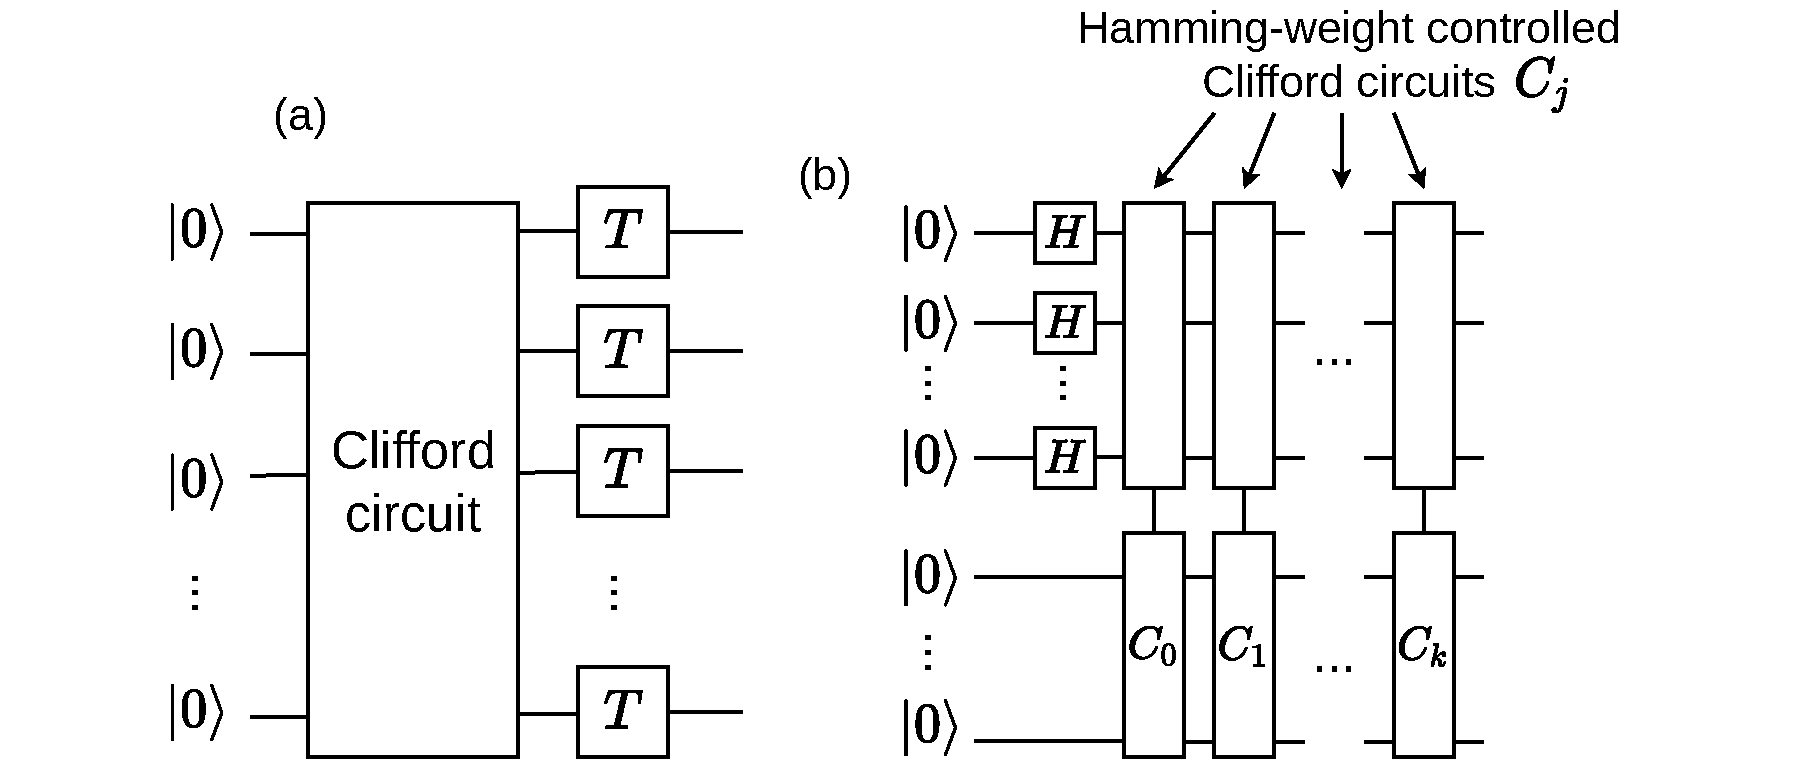
\includegraphics[width=1.0\textwidth]{pics/t-gate-tower.pdf}
	\caption{
		Circuits output a polynomially-size \limdd.
		For (b), the Hamming-weight controlled-$C$ gate on $c$ control qubits and $t$ target qubits maps $\ket{x}\otimes \ket{y}$ to $\ket{x}\otimes C\ket{y}$ if $|x| = 1$ and to $\ket{x}\otimes\ket{y}$ otherwise, for $x\in \{0, 1\}^c$ and $y\in \{0, 1\}^t$.
		Here, $|x| = \sum_{j=1}^c x_j$ denotes the Hamming weight of $x$.
		\todo[inline]{need to explain how to implement Hamming-weight controlled gate?}
		\label{fig:stabilizer-rank-hard}
	}
\end{figure}

